% Options for packages loaded elsewhere
\PassOptionsToPackage{unicode}{hyperref}
\PassOptionsToPackage{hyphens}{url}
%
\documentclass[
]{article}
\usepackage{lmodern}
\usepackage{amssymb,amsmath}
\usepackage{ifxetex,ifluatex}
\ifnum 0\ifxetex 1\fi\ifluatex 1\fi=0 % if pdftex
  \usepackage[T1]{fontenc}
  \usepackage[utf8]{inputenc}
  \usepackage{textcomp} % provide euro and other symbols
\else % if luatex or xetex
  \usepackage{unicode-math}
  \defaultfontfeatures{Scale=MatchLowercase}
  \defaultfontfeatures[\rmfamily]{Ligatures=TeX,Scale=1}
\fi
% Use upquote if available, for straight quotes in verbatim environments
\IfFileExists{upquote.sty}{\usepackage{upquote}}{}
\IfFileExists{microtype.sty}{% use microtype if available
  \usepackage[]{microtype}
  \UseMicrotypeSet[protrusion]{basicmath} % disable protrusion for tt fonts
}{}
\makeatletter
\@ifundefined{KOMAClassName}{% if non-KOMA class
  \IfFileExists{parskip.sty}{%
    \usepackage{parskip}
  }{% else
    \setlength{\parindent}{0pt}
    \setlength{\parskip}{6pt plus 2pt minus 1pt}}
}{% if KOMA class
  \KOMAoptions{parskip=half}}
\makeatother
\usepackage{xcolor}
\IfFileExists{xurl.sty}{\usepackage{xurl}}{} % add URL line breaks if available
\IfFileExists{bookmark.sty}{\usepackage{bookmark}}{\usepackage{hyperref}}
\hypersetup{
  pdftitle={Public Indebtedness and Foreign Credit Demand for Emerging Bonds},
  pdfauthor={Augusto Netto, Gabriella Garcia and Maria Clara Drzeviechi},
  hidelinks,
  pdfcreator={LaTeX via pandoc}}
\urlstyle{same} % disable monospaced font for URLs
\usepackage[margin=1in]{geometry}
\usepackage{color}
\usepackage{fancyvrb}
\newcommand{\VerbBar}{|}
\newcommand{\VERB}{\Verb[commandchars=\\\{\}]}
\DefineVerbatimEnvironment{Highlighting}{Verbatim}{commandchars=\\\{\}}
% Add ',fontsize=\small' for more characters per line
\usepackage{framed}
\definecolor{shadecolor}{RGB}{248,248,248}
\newenvironment{Shaded}{\begin{snugshade}}{\end{snugshade}}
\newcommand{\AlertTok}[1]{\textcolor[rgb]{0.94,0.16,0.16}{#1}}
\newcommand{\AnnotationTok}[1]{\textcolor[rgb]{0.56,0.35,0.01}{\textbf{\textit{#1}}}}
\newcommand{\AttributeTok}[1]{\textcolor[rgb]{0.77,0.63,0.00}{#1}}
\newcommand{\BaseNTok}[1]{\textcolor[rgb]{0.00,0.00,0.81}{#1}}
\newcommand{\BuiltInTok}[1]{#1}
\newcommand{\CharTok}[1]{\textcolor[rgb]{0.31,0.60,0.02}{#1}}
\newcommand{\CommentTok}[1]{\textcolor[rgb]{0.56,0.35,0.01}{\textit{#1}}}
\newcommand{\CommentVarTok}[1]{\textcolor[rgb]{0.56,0.35,0.01}{\textbf{\textit{#1}}}}
\newcommand{\ConstantTok}[1]{\textcolor[rgb]{0.00,0.00,0.00}{#1}}
\newcommand{\ControlFlowTok}[1]{\textcolor[rgb]{0.13,0.29,0.53}{\textbf{#1}}}
\newcommand{\DataTypeTok}[1]{\textcolor[rgb]{0.13,0.29,0.53}{#1}}
\newcommand{\DecValTok}[1]{\textcolor[rgb]{0.00,0.00,0.81}{#1}}
\newcommand{\DocumentationTok}[1]{\textcolor[rgb]{0.56,0.35,0.01}{\textbf{\textit{#1}}}}
\newcommand{\ErrorTok}[1]{\textcolor[rgb]{0.64,0.00,0.00}{\textbf{#1}}}
\newcommand{\ExtensionTok}[1]{#1}
\newcommand{\FloatTok}[1]{\textcolor[rgb]{0.00,0.00,0.81}{#1}}
\newcommand{\FunctionTok}[1]{\textcolor[rgb]{0.00,0.00,0.00}{#1}}
\newcommand{\ImportTok}[1]{#1}
\newcommand{\InformationTok}[1]{\textcolor[rgb]{0.56,0.35,0.01}{\textbf{\textit{#1}}}}
\newcommand{\KeywordTok}[1]{\textcolor[rgb]{0.13,0.29,0.53}{\textbf{#1}}}
\newcommand{\NormalTok}[1]{#1}
\newcommand{\OperatorTok}[1]{\textcolor[rgb]{0.81,0.36,0.00}{\textbf{#1}}}
\newcommand{\OtherTok}[1]{\textcolor[rgb]{0.56,0.35,0.01}{#1}}
\newcommand{\PreprocessorTok}[1]{\textcolor[rgb]{0.56,0.35,0.01}{\textit{#1}}}
\newcommand{\RegionMarkerTok}[1]{#1}
\newcommand{\SpecialCharTok}[1]{\textcolor[rgb]{0.00,0.00,0.00}{#1}}
\newcommand{\SpecialStringTok}[1]{\textcolor[rgb]{0.31,0.60,0.02}{#1}}
\newcommand{\StringTok}[1]{\textcolor[rgb]{0.31,0.60,0.02}{#1}}
\newcommand{\VariableTok}[1]{\textcolor[rgb]{0.00,0.00,0.00}{#1}}
\newcommand{\VerbatimStringTok}[1]{\textcolor[rgb]{0.31,0.60,0.02}{#1}}
\newcommand{\WarningTok}[1]{\textcolor[rgb]{0.56,0.35,0.01}{\textbf{\textit{#1}}}}
\usepackage{graphicx,grffile}
\makeatletter
\def\maxwidth{\ifdim\Gin@nat@width>\linewidth\linewidth\else\Gin@nat@width\fi}
\def\maxheight{\ifdim\Gin@nat@height>\textheight\textheight\else\Gin@nat@height\fi}
\makeatother
% Scale images if necessary, so that they will not overflow the page
% margins by default, and it is still possible to overwrite the defaults
% using explicit options in \includegraphics[width, height, ...]{}
\setkeys{Gin}{width=\maxwidth,height=\maxheight,keepaspectratio}
% Set default figure placement to htbp
\makeatletter
\def\fps@figure{htbp}
\makeatother
\setlength{\emergencystretch}{3em} % prevent overfull lines
\providecommand{\tightlist}{%
  \setlength{\itemsep}{0pt}\setlength{\parskip}{0pt}}
\setcounter{secnumdepth}{-\maxdimen} % remove section numbering

\title{Public Indebtedness and Foreign Credit Demand for Emerging Bonds}
\author{Augusto Netto, Gabriella Garcia and Maria Clara Drzeviechi}
\date{}

\begin{document}
\maketitle

{
\setcounter{tocdepth}{2}
\tableofcontents
}
\textbf{Insper Data}

\hypertarget{objective}{%
\section{Objective}\label{objective}}

This study aims to investigate the economic determinants of foreign
participation in a country's public debt. Investors, when allocating
resources in foreign countries, can look for different things such as
stability, higher returns or just diversification of assets. Each
country can serve to fulfill one of these objectives and, depending on
the macroeconomic fundamentals, they can be more or less attractive to
investors. In addition, it is necessary to analyze emerging and advanced
countries separately, considering that these two groups have very
divergent characteristics. Thus, this work wants to understand which are
the macroeconomic determinants that can attract or put away bondholders,
for both advanced or emerging countries.

\hypertarget{introduction}{%
\section{Introduction}\label{introduction}}

In the past 50 years, emerging and developing economies experienced four
big indebtedness waves, three of which ended up in financial crises. In
the 1980s, the association of low real interest rates and growing debt
market led certain economies to raise considerably their levels of
indebtedness; the result was the well-known Latin America's debt crisis.
A decade later, the world would watch the Asian financial crisis, due to
the liberalization of financial markets and capital flows, allowing
these countries to acquire loans in foreign currencies. Finally, in
2007-09, both emerging and advanced economies faced major recessions as
a result of the global financial crisis.

It is important to notice that although happening in different decades
and locations, these three episodes share a common denominator: they all
started in periods with low real interest rates and an escalating
indebtedness. This scenario made the risk premium rise and subsequently
there was a sudden stop of capital flows.

In 2010, the fourth global wave of debt started, and it was the largest
and fastest one. In accordance with the aforementioned ones, interest
rates were low since the Global Financial Crisis and investors were
seeking assets with greater profitability. It is also reasonable to
consider that this wave has not yet met its end. By 2018, according to
the IMF, global debt has reached 226\% of GDP, representing an amount of
188 trillions of dollars. Emerging and developing economies saw
indebtedness grow 54 p.p. in 8 years, reaching 170\% of GDP. Low income
countries reached 67\% of GDP in 2018 -- that figure was 48\% in 2010. A
different situation is seen on advanced economies, once they have
maintained the 265\% ratio of debt to GDP on the same level since 2010.

Global debt waves have shown the need for emerging and developing
markets to develop their sovereign bond markets to facilitate public
debt financing and management, primarily through the issuance of
domestic bonds in local currencies. This growth was reflected in the
increase in domestic participation in government bonds, and in the
increase in foreign interest in the debt of these governments, which has
become increasingly relevant in the local bond market.

The raise in foreign participation in the sovereign debt market is also
related to many susceptible advantages, such as a decrease in government
borrowing costs, due to the higher demand for these bonds, presented in
several studies (Andritzky, 2012; Arslanalp and Poghosyan, 2014;
Jaramillo and Zhang, 2013; Warnock and Warnock, 2009) and the
diversification of the investor base, reflecting different
characteristics of investors in terms of risk tolerance and trading
reasons, which may increase the liquidity of government debt bonds in
the secondary market (World Bank and IMF , 2001).

However, foreign investors tend to be relatively more sensitive to risk,
particularly foreign private investors, and can be an unstable source of
demand in times of stress, because they have a broader pool of assets in
which they can invest. As a result, they may be less inclined to
maintain their participation during these episodes (Broner et al.,
2013).

The constant rise in indebtedness, observed in the current wave of
global debt and intensified by the current crisis of COVID-19, may
culminate in a sudden increase in risk premiums, if investors consider
debt to GDP levels to be unsustainable (Blanchard 2019; Henderson 2019;
Rogoff 2019a, b). If this happens, both capital inflows and outflows
decrease during economic crises, with this effect being stronger in
global crises (Broner et al., 2013).

In this context, this study aims to analyze the different impacts of
public debt on the participation of foreign creditors in government
bonds, depending on different scenarios and macroeconomic fundamentals.
Given the negative relationship between the level of public debt and
foreign investors already explored in the literature, we will
investigate how this effect varies over time and conditions.

Therefore, a worldwide analysis will be conducted using the database
provided by Arslanalp and Takahiro Tsuda, previously affiliated with the
Monetary and Capital Markets Department of the International Monetary
Fund.

\hypertarget{literature-review}{%
\section{Literature Review}\label{literature-review}}

Discussions on how indebtedness can affect the macroeconomic variables
of a country are widely addressed in the literature. The main topics are
related to foreign investors; growth; debt overhang and debt tolerance.

More initially, countries' ability to attract non-local investors was
studied by Burger and Warnok (2005). The study showed that countries
with a history of low inflation tend to have a more developed bond
market. Subsequently, Brutti and Sauré (2012) studied the importance of
a derivatives market for the quality of a bond market.

In this study, it is important to highlight the developed literature
Arslanap and Tsuda (2014). The authors, in addition to having compiled
the database used in this article, carried out several analyzes on
foreign participation in the bond market. It was noted that, as of 2010,
there was a great flow of foreign capital to the emerging securities
market. In addition, they concluded that countries with a lower
debt-to-GDP rate are more attractive to foreign investors.

The relationship between debt and growth was first found to be
non-linear by Reinhart, Rogoff, and Savastano (2003). Later, Reinhart
and Rogoff (2010) analyze countries distinguishing developed and
emerging markets and they found out that, for both groups, a 90\% debt
to GDP ratio can be detrimental for growth. On the other hand, Kumar and
Woo (2010) produced evidence that the negative impact of debt on growth
is higher for developing countries when compared with developed
countries.

Thinking about debt tolerance, Reinhart, Rogoff and Savastano (2003)
introduce the concept of debt intolerance and analyze how emerging
markets find it difficult to face high levels of debt, while advanced
countries face this issue more easily. Later, Catão and Kapur (2006)
discussed the macroeconomic determinants of a country's volatility and
how it impacts the spread rate it has to pay.

The concept of debt overhang refers to a debt burden so large that the
country can not take any additional debt to finance itself. Krugman
(1988) discussed the tradeoff for creditors when facing a debt overhang:
financing or forgiving. Deshpande (1995) discusses how a situation of
debt overhang can discourage investment. Reinhart, Reinhart, and Rogoff
(2012) punctuated the main episodes in history about debt overhang.

\hypertarget{dataset}{%
\section{Dataset}\label{dataset}}

The dataset used in this study is composed by the database provided by
Arslanalp and Takahiro Tsuda, previously affiliated with the Monetary
and Capital Markets Department of the International Monetary Fund.
Arslanalp and Takahiro Tsuda provide estimates of investor holdings of
government debt of 24 advanced economies and 24 emerging market
economies.

The investor base is grouped under six classes: domestic central bank,
domestic banks, domestic nonbanks, foreign official sector, foreign
banks, and foreign nonbanks. Banks include depository institutions other
than central banks, based on the definition used in the IMF's
International Financial Statistics (IFS). Nonbanks include other
investors, including insurance companies, pension funds, and investment
funds. Investment funds could be mutual funds, exchange-traded funds
(ETFs), or sovereign wealth funds (SWFs). The foreign official sector
for Emerging Markets includes official loans and foreign central bank
holdings of EM government debt as reserve assets, and for Advanced
Markets includes foreign central banks and other foreign official
creditors.

For this study, 45 of the 48 countries present at the base of Arslanalp
and Tsuda are used. The data are annualized through the fourth quarter
of each year and the sample period used covers the years 2004 to 2019.

Macroeconomic and financial data were obtained from the World Economic
Outlook Database published by the International Monetary Fund in April
2020. For countries where the nominal interest rate was incomplete on
the basis of the IMF, the missing data was obtained on the website of
the central banks in each country.

\hypertarget{stylized-facts-about-the-database}{%
\section{Stylized facts about the
database}\label{stylized-facts-about-the-database}}

Given the recovery of economies affected by the Asian financial crisis
(1990s), global indebtedness resumed at an accelerated pace. This
coincided with a period of rapid expansion for banks based in the United
States and the European Union (Arteta and Kasyanenko 2019). The third
global debt wave that started in 2002 was represented by a sharp
increase in loans from emerging markets in international debt markets,
due to low global interest rates. In 2004, 6 emerging markets were among
the 10 countries with the highest levels of debt to GDP (graph 1). In
contrast, emerging markets had the largest share of foreign investors,
in 2004, they were not the most indebted countries (graph 2).

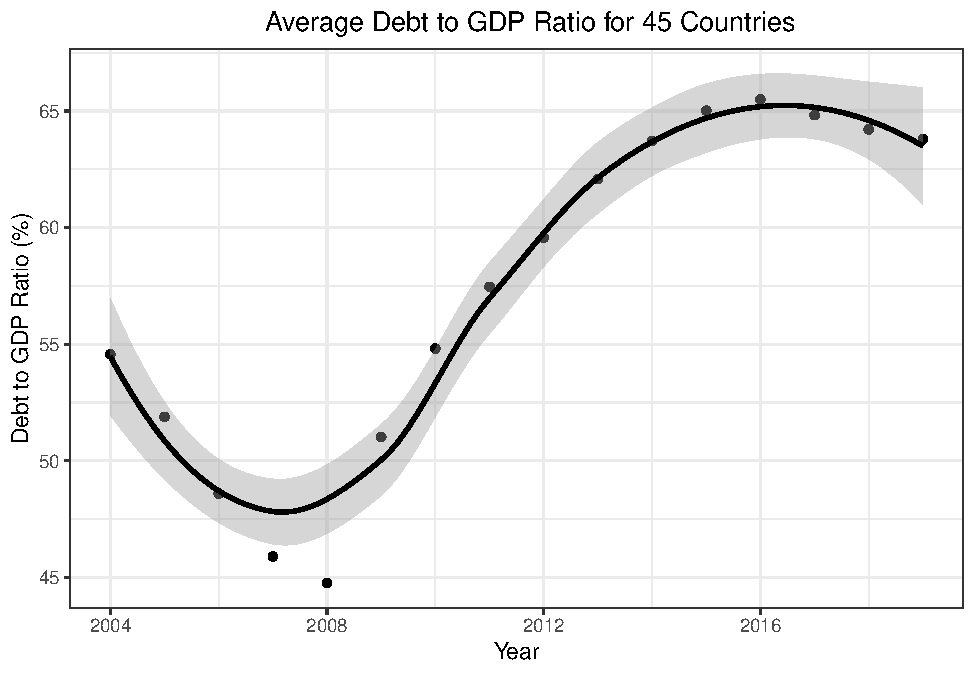
\includegraphics{final_project_files/figure-latex/unnamed-chunk-2-1.pdf}
\includegraphics{final_project_files/figure-latex/unnamed-chunk-2-2.pdf}

In addition, low inflation and fiscal stabilization in many emerging
markets have contributed to an increase in the credibility of
macroeconomic policies (Kose and Ohnsorge, 2019), contributing to the
development of the bond market in these countries. Thus, the third wave
of debt had a lesser effect on the emerging markets, which even showed a
reversal in the level of debt over GDP, given the improvement in fiscal
balances and debt management, which lasted until the period of the
global financial crisis. (graph 3).

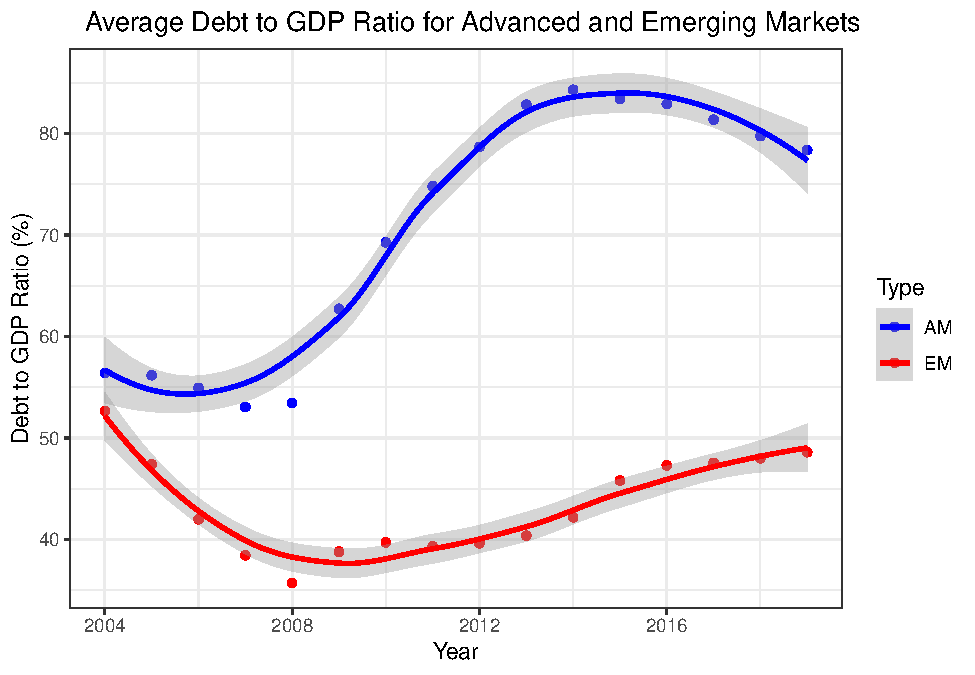
\includegraphics{final_project_files/figure-latex/unnamed-chunk-3-1.pdf}

In 2010, the fourth and current global debt wave began, its
characteristics are similar to the previous ones, low global interest
rates (graph 4) and changes in the financial markets that allowed for
rapid debt contraction in both advanced and emerging markets. In 2009,
emerging markets debt to GDP averaged 38 percent of GDP reaching 48
percent at the end of 2019, while advanced markets grew by around 30
percentage points between 2008 and 2014 when they peaked at an average
of 84 percent of GDP (graph 3).

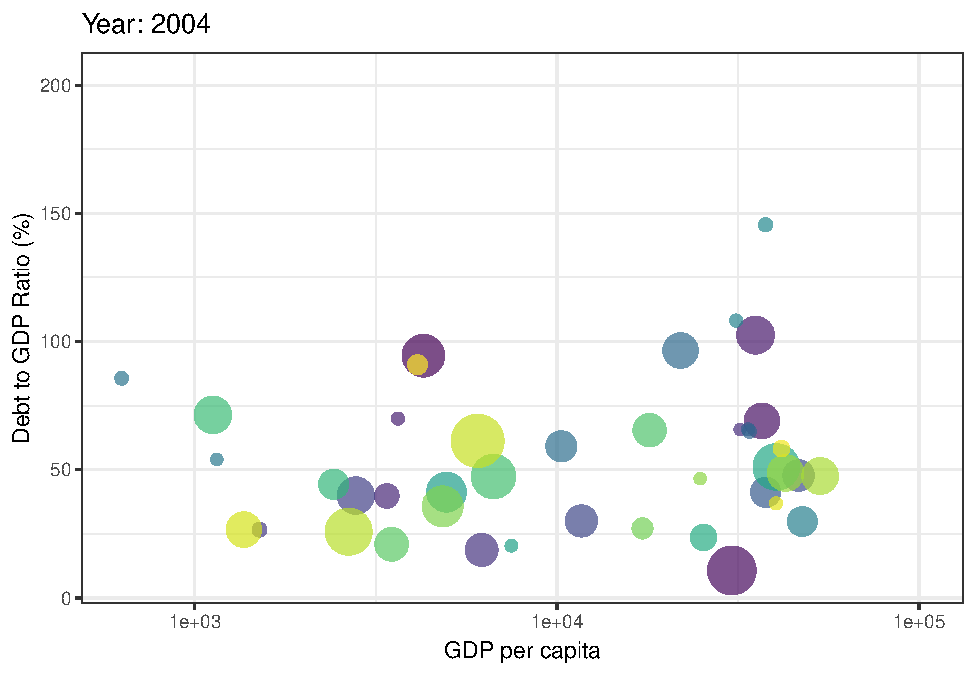
\includegraphics{final_project_files/figure-latex/unnamed-chunk-4-1.pdf}

Foreign participation in domestic public debt, since 2005, is higher in
advanced markets, due to the greater financial strength and credibility
of these countries, therefore, foreign investors are more willing to
access these markets (graph 5). In addition, advanced markets are more
tolerant of foreign participation because there are rarely abrupt
reversals of capital, as in emerging countries.

\includegraphics{final_project_files/figure-latex/unnamed-chunk-5-1.pdf}

The 2008 global financial crisis caused a sharp rise in aversion to
global risks, as well as a reduction in international liquidity. As a
result, there was a reversal of capital flows to secure markets in
emerging markets and, consequently, a reduction in foreign participation
in these markets, which had been observed since 2004 (graph 5). However,
shortly after the crisis, international flows to emerging countries
resumed, with the result that governments in emerging markets
considerably increased the issuance of sovereign debt securities, and
consequently increased foreign participation in the local debt market,
however, making those countries most vulnerable to shocks in investor
confidence.

\hypertarget{other-descriptive-analysis}{%
\section{Other descriptive analysis}\label{other-descriptive-analysis}}

\hypertarget{evolution-of-public-debt-in-emerging-markets}{%
\subsection{Evolution of public debt in emerging
markets}\label{evolution-of-public-debt-in-emerging-markets}}

\includegraphics{final_project_files/figure-latex/unnamed-chunk-6-1.pdf}
\includegraphics{final_project_files/figure-latex/unnamed-chunk-6-2.pdf}
\includegraphics{final_project_files/figure-latex/unnamed-chunk-6-3.pdf}

\hypertarget{evolution-of-the-participation-of-foreign-investors-in-government-debt-in-emerging-markets}{%
\subsection{Evolution of the participation of foreign investors in
government debt in Emerging
Markets}\label{evolution-of-the-participation-of-foreign-investors-in-government-debt-in-emerging-markets}}

\includegraphics{final_project_files/figure-latex/unnamed-chunk-7-1.pdf}
\includegraphics{final_project_files/figure-latex/unnamed-chunk-7-2.pdf}
\includegraphics{final_project_files/figure-latex/unnamed-chunk-7-3.pdf}

\hypertarget{countries-have-different-indebtedness-levels}{%
\subsection{Countries have different indebtedness
levels}\label{countries-have-different-indebtedness-levels}}

\includegraphics{final_project_files/figure-latex/unnamed-chunk-8-1.pdf}

As the map shown above makes clear, countries around the world have
contrasting levels of debt to GDP. Nations in grey are not part of our
sample.

\hypertarget{foreign-investors-have-a-preference-for-allocating-their-resources-in-advanced-markets}{%
\subsubsection{Foreign investors have a preference for allocating their
resources in advanced
markets}\label{foreign-investors-have-a-preference-for-allocating-their-resources-in-advanced-markets}}

\includegraphics{final_project_files/figure-latex/unnamed-chunk-9-1.pdf}

It is possible to observe that foreign investors have allocated much
more resources in bonds from advanced markets.

\hypertarget{the-participation-of-domestic-investors-in-the-composition-of-debt-it-is-not-invariant-over-time}{%
\subsubsection{The participation of domestic investors in the
composition of debt it is not invariant over
time}\label{the-participation-of-domestic-investors-in-the-composition-of-debt-it-is-not-invariant-over-time}}

\includegraphics{final_project_files/figure-latex/unnamed-chunk-10-1.pdf}

In addition to the domestic participation in debt varying for both
emerging and advanced countries, it is possible to infer that those
variations are inverse.

\hypertarget{there-is-no-clear-relationship-between-participation-of-foreign-investor-in-government-debt-and-inflation}{%
\subsubsection{There is no clear relationship between participation of
foreign investor in government debt and
inflation}\label{there-is-no-clear-relationship-between-participation-of-foreign-investor-in-government-debt-and-inflation}}

\includegraphics{final_project_files/figure-latex/unnamed-chunk-11-1.pdf}

\hypertarget{there-is-no-clear-relationship-between-the-participation-of-foreign-investor-in-government-debt-and-nominal-interest-rate}{%
\subsubsection{There is no clear relationship between the participation
of foreign investor in government debt and nominal interest
rate}\label{there-is-no-clear-relationship-between-the-participation-of-foreign-investor-in-government-debt-and-nominal-interest-rate}}

\includegraphics{final_project_files/figure-latex/unnamed-chunk-12-1.pdf}

\begin{Shaded}
\begin{Highlighting}[]
\CommentTok{#install.packages("gifski") #if not already installed}
\CommentTok{# library(gifski)}

\CommentTok{# animated <- dataset_total %>% }
\CommentTok{#  mutate(share = (nonbank_foreign_debt + bank_foreign_debt)/total_debt) %>%}
\CommentTok{#  group_by(country, yearnum) %>% }
\CommentTok{#  mutate(media_debt_GDP = mean(debt_to_GDP)) %>% }
\CommentTok{#  ggplot() +}
\CommentTok{#  geom_point(aes(x = debt_to_GDP, y = share), colour = "black") +}
\CommentTok{#  geom_text(aes(x = debt_to_GDP, y = share, colour = country, label = country, fontface = 2),}
\CommentTok{#            hjust = 0.5, vjust = -0.5, size = 3) +}
\CommentTok{#  theme_bw() +}
\CommentTok{#  theme(legend.position = "none", plot.title = element_text(size = 15)) +}
\CommentTok{#  xlab("Dívida/PIB") +}
\CommentTok{#  ylab("% Investidores estrangeiros")}

\CommentTok{#(gif_debt <- animated + transition_time(yearnum) +}
\CommentTok{#  labs(title = "Year: \{frame_time\}"))}

\CommentTok{#anim_save("filenamehere.gif", gif_debt)}
\end{Highlighting}
\end{Shaded}

\hypertarget{methodology}{%
\subsection{Methodology}\label{methodology}}

The methodology used in this study will consist of regressions with
panel data. Within and pooled models will be used and compared in order
to obtain the most appropriate model. The advantages of using panel data
are the possibility to follow the evolution of several countries over
time, being able to capture the specific effects of each country and
each period of time. In addition, the database was divided between
emerging and advanced countries, with the objective of carrying out
econometric analysis for these two groups separately.

The regression response variable will be the proportion of foreign
participation in the total debt issued by a given country, excluding
official institutions. Regarding the explanatory variables are,
essentially, macroeconomic fundamentals, such as inflation, policy rate,
debt-to-GDP-ratio, the balance of payments, exchange rate volatility,
and others. Moreover, dummies to control specific periods of the economy
will be included in the model.

The specification of the main model must follow the following equation:

\[ \%\;External\;Investors_{it} = \alpha_i \;+ \;\sum{\beta_n \cdot Macro\; Determinants_{it}}\; + \;\sum{\beta_k \cdot Period\;Dummy_{it}} \;\;\;\;\; (1)\]

\[\%\;External\;Investors_{it} = \alpha_t \;+ \;\sum{\beta_n \cdot Macro\; Determinants_{it}}\; + \;\sum{\beta_k \cdot Period\;Dummy_{it}} \;\;\;\;\; (2)\]
\[\%\;External\;Investors_{it} = \alpha_{it} \;+ \;\sum{\beta_n \cdot Macro\; Determinants_{it}}\; + \;\sum{\beta_k \cdot Period\;Dummy_{it}} \;\;\;\;\; (3)\]
\[\%\;External\;Investors_{it} = \alpha \;+ \;\sum{\beta_n \cdot Macro\; Determinants_{it}}\; + \;\sum{\beta_k \cdot Period\;Dummy_{it}} \;\;\;\;\; (4)\]

As one can see in equations (1) to (4), we ran models with different
effects. Model (1) uses country fixed effects; model (2), year fixed
effect; model (3), both country and year fixed effect; and lastly model
(4) is a pooled cross-section.

Also, the percentage of external investors goes for the participation of
foreigners in the local debt, excluding official institutions - such as
Central Banks. We tested a variety of macro determinants: debt to GDP,
log of GDP per capita, nominal interest rate, FX volatility, account
balance, lend/borrow rate and VIX EUA.

\hypertarget{econometric-results}{%
\subsection{Econometric results}\label{econometric-results}}

\hypertarget{regression-results-for-advanced-markets}{%
\subsubsection{Regression Results for Advanced
Markets}\label{regression-results-for-advanced-markets}}

\begin{verbatim}
## 
## Advanced Markets
## ==============================================================
##                                  Dependent variable:          
##                        ---------------------------------------
##                         Foreign participation on public debt  
##                           (1)        (2)       (3)      (4)   
## --------------------------------------------------------------
## debt_to_GDP              0.001     0.0003    0.0005    0.0003 
##                         (0.001)    (0.001)   (0.001)  (0.001) 
##                                                               
## post_08YES               0.041                         -0.052 
##                         (0.031)                       (0.056) 
##                                                               
## ln_GDP_per_cap_cte       -0.002     0.001    -0.002    0.002  
##                         (0.001)    (0.003)   (0.001)  (0.003) 
##                                                               
## nominal_rate            0.018***    0.001    0.018**  -0.0003 
##                         (0.007)    (0.011)   (0.008)  (0.010) 
##                                                               
## lending_borroeing_rate -0.007***  -0.007**  -0.005**  -0.007**
##                         (0.002)    (0.003)   (0.002)  (0.003) 
##                                                               
## vix_EUA                  0.001                         0.003  
##                         (0.001)                       (0.003) 
##                                                               
## debt_to_GDP:post_08YES -0.001***   -0.001   -0.001***  -0.001 
##                         (0.0003)   (0.001)  (0.0003)  (0.001) 
##                                                               
## Constant                                              0.216***
##                                                       (0.064) 
##                                                               
## --------------------------------------------------------------
## Country FE                YES        NO        YES       NO   
## Year FE                    NO        YES       YES       NO   
## Observations              285        285       285      285   
## R2                       0.267      0.021     0.103    0.077  
## Adjusted R2              0.186     -0.053    -0.049    0.053  
## ==============================================================
## Note:                              *p<0.1; **p<0.05; ***p<0.01
\end{verbatim}

In view of the results, we must pay attention to those that proved to be
significant in our model. Regarding the interest rate, it shows to have
a positive effect, when significant, indicating that higher returns
attract investors. The lending-borrowing rate has a negative effect,
indicating that advanced countries that are creditors to the world
receive a smaller flow of foreign capital. And, finally, we have the
impact of the interaction between debt-to-GDP ratio and the `post 2008'
dummy with a negative effect, indicating a negative capital flow in post
2008 for advanced countries already more indebted.

\hypertarget{regression-results-for-emerging-markets}{%
\subsubsection{Regression Results for Emerging
Markets}\label{regression-results-for-emerging-markets}}

\begin{verbatim}
## 
## Emerging Markets - Threshold comparison
## ==========================================================
##                              Dependent variable:          
##                    ---------------------------------------
##                     Foreign participation on public debt  
##                       (1)        (2)      (3)       (4)   
## ----------------------------------------------------------
## debt_to_GDP         -0.0004   -0.001***  -0.001  -0.001***
##                     (0.0003)  (0.0003)  (0.0003) (0.0003) 
##                                                           
## post_08YES          0.043***                       0.024  
##                     (0.009)                       (0.017) 
##                                                           
## ln_GDP_per_cap_cte   0.002     -0.002    0.002    -0.002  
##                     (0.001)    (0.003)  (0.001)   (0.003) 
##                                                           
## nominal_rate         -0.001   -0.004**  -0.002** -0.003** 
##                     (0.001)    (0.001)  (0.001)   (0.001) 
##                                                           
## fx_volatility       -0.00001   0.00003  -0.00002  0.00002 
##                     (0.0001)  (0.00005) (0.0001) (0.00005)
##                                                           
## account_balance      -0.001   -0.006***  -0.001  -0.006***
##                     (0.001)    (0.001)  (0.001)   (0.001) 
##                                                           
## vix_EUA            -0.004***                     -0.005***
##                     (0.001)                       (0.001) 
##                                                           
## Constant                                         0.355*** 
##                                                   (0.034) 
##                                                           
## ----------------------------------------------------------
## Country FE            YES        NO       YES       NO    
## Year FE                NO        YES      YES       NO    
## Observations          290        290      290       290   
## R2                   0.159      0.133    0.034     0.167  
## Adjusted R2          0.068      0.069    -0.126    0.147  
## ==========================================================
## Note:                          *p<0.1; **p<0.05; ***p<0.01
\end{verbatim}

A very similar regression specification was utilized for the subset of
emerging markets. As we already expected, the effects of macroeconomic
variables in the participation of foreign investors is largely different
from the results seen for advanced economies. First of all, a rise in
the debt to GDP level is expected to pull away foreign participation,
regardless of the global economy momentum, which is logical and seems to
corroborate with the idea of debt intolerance experienced by emerging
markets (Reinhart et. al.~2003). At the same time, through a dummy
variable indicating the period after the global financial crisis in
2008, we can see that the ammount of debt held by foreigners rose in
average after 2008.

Finally, it is specially worth of mentioning that, according to our
results, one should not expect a rise in foreign share through higher
policy rates, which seems to defy the common knowledge, but, as a sort
of mirror from what we have found for advanced markets, higher levels of
volatility repels the investors from emerging economies to the safer and
more advanced ones.

\hypertarget{concluding-remarks}{%
\subsubsection{Concluding remarks}\label{concluding-remarks}}

\hypertarget{references}{%
\section{References}\label{references}}

REFERENCES:

Andritzky, J. R., 2012, ``Government Bonds and Their Investors: What Are
the Facts and Do They Matter?'' IMF Working Paper No.~12/158
(Washington: International Monetary Fund).

Arslanalp, S. and T. Poghosyan, 2014, ``Foreign Investor Flows and
Sovereign Bond Yields in Advanced Economies'' IMF Working Paper 14/27
(Washington: International Monetary Fund).

Arslanalp, S., and Tsuda, T. ``Tracking Global Demand for Emerging
Market Sovereign Debt'' IMF working papers (2014): 14/39

---------, and ---------. ``Tracking Global Demand for Advanced Economy
Sovereign Debt'' IMF working papers (2012): 12/284

Blanchard, O. J., and L. H. Summers. 2019. Evolution or Revolution?
Rethinking Macroeconomic Policy After the Great Recession. Cambridge:
MIT Press. Broner, F., T. Didier, A. Erce, and S. Schmukler, (2013).
``Gross capital flows: Dynamics and crises'', Journal of Monetary
Economics 60, 113-33 Catão, Luis, and Sandeep Kapur. ``Volatility and
the debt-intolerance paradox.'' IMF Staff Papers 53.2 (2006): 195-218.

Deshpande, Ashwini. ``The debt overhang and the disincentive to
invest.'' Journal of development Economics 52.1 (1997): 169-187.
Jaramillo L., and S. Zhang, 2013, ``Real Money Investors and Sovereign
Bond Yields,'' IMF Working Paper No.~12/158, (Washington: International
Monetary Fund). Krugman, Paul R. Financing vs.~forgiving a debt
overhang. No.~w2486. National Bureau of Economic Research, 1988.

Kumar, Manmohan, and Jaejoon Woo. ``Public debt and growth.'' IMF
working papers (2010): 1-47.

Reinhart, Carmen M., and Kenneth S. Rogoff. ``Growth in a Time of
Debt.'' American economic review 100.2 (2010): 573-78.

Reinhart, Carmen M., Kenneth S. Rogoff, and Miguel A. Savastano. Debt
intolerance. No.~w9908. National Bureau of Economic Research, 2003.

Reinhart, Carmen M., Vincent R. Reinhart, and Kenneth S. Rogoff.
``Public debt overhangs: advanced-economy episodes since 1800.'' Journal
of Economic Perspectives 26.3 (2012): 69-86.

Rogoff, K. 2019a. ``Risks to the Global Economy in 2019.'' Project
Syndicate, January 11.
\url{https://www.project-syndicate.org/commentary/global-economy-mainrisks-in-2019-by-kenneth-rogoff-2019-01}.

---------. 2019b. ``Government Debt is Not A Free Lunch .'' Project
Syndicate, December 6.
\url{https://www.project-syndicate.org/commentary/government-debt-lowinterest-rates-no-free-lunch-by-kenneth-rogoff-2019-11}
.

Burger, J., and Warnock, F. (2006). ``Local Currency Bond Markets'', IMF
Staff Papers, 53: pp.~133--146.

World Bank and International Monetary Fund, 2001, ``Developing
Government Bond Markets: A Handbook,'' World Bank Publications
(Washington: International Monetary Fund).

\end{document}
